\section{Custom PGM to OBJ converter}
GMapping creates a PGM file, which is an image format. This is in 2D because GMapping can only create 2D maps. Recast is however perfectly capable of performing calculations on 3D maps, as it is designed to be used in a gaming environment. This however means that the input for Recast needs to be in 3D format, so a converter of PGM to OBJ was needed. The basic idea behind this converter is that each black pixel in the PGM file (which represents a wall or obstacle of some sort) gets converted to a rectangle with a good height in 3D. This height needs to be larger than the height of the agent in Recast, or else Recast will think it can climb over this rectangle. Each white pixel, which represents a flat surface in 2D, needs to be converted to a flat square. In order to make this conversion respectably compact, in a short amount of time, each line in the PGM image is scanned. All consecutive white or black pixels are converted to rectangles, instead of converting every pixel to a separate square. If later on a 3D mapping algorithm is used, Recast does not need to be adjusted, at most a new converter has to be written if this algorithm does not output OBJ files.

The result of converting a map of a home environment map to an OBJ file can be seen in figure \ref{fig:navigation_mesh}.

\begin{figure}[ht!]
	\centering
	\mbox{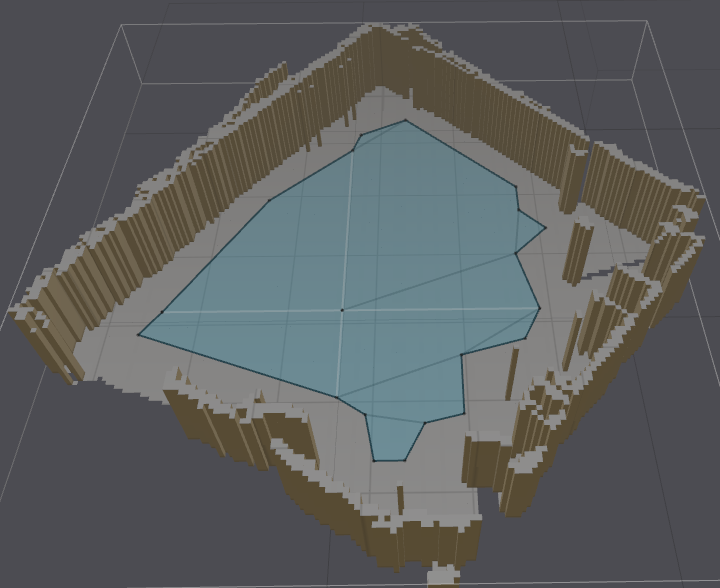
\includegraphics[scale=0.2]{Images/navigation_mesh.png}}
	\caption{A navigation mesh of a home environment generated using Recast.}
	\label{fig:navigation_mesh}
\end{figure}

This figure also shows the navigation mesh mentioned earlier. For 2D environments, this navigation mesh is basically the flat surface which is then eroded by the radius of the agent (in this case Eva). If the map was created in 3D, Recast could also determine which slopes the agent can drive up and which obstacles it can drive over.

\section{Path handler}
The path handler works almost as a spring would, where the spring would follow the ideal path calculated. If the angle between Eva and the focal point is too large (currently set at $\frac{1}{6}\pi$), it will only make Eva rotate. If the angle between Eva and the focal point is between $0$ and $\frac{1}{6}\pi$, the angular speed gets scaled (at 0 angle it is completely off, at $\frac{1}{6}\pi$ it is fully rotating) and the linear speed gets scaled twice; once depending on how far Eva is from her target (scaling begins from 3 meters away and stops at 1 meter) and once depending on how fast she wants to rotate.

In formula form, the linear speed is:
\begin{align*}
	path\_scale& = max(min(remaining\_path\_length, 3.0), 1.0) - 1.0) / 2.0 \\
	angular\_scale& = 1.0 - min(\frac{abs(angle\_to\_focal)}{\frac{1}{6}\pi}, 1.0) \\
	linear\_speed& = angular\_scale * (path\_scale * (max\_linear - min\_linear) + min\_linear) \\
\end{align*}

And the angular speed:
\begin{align*}
	scale& = min(\frac{abs(angle\_to\_focal)}{\frac{1}{6}\pi}, 1.0) \\
	angular\_speed& = scale * max\_angular
\end{align*}

The focal point is set to be a certain distance (0.5m proved to be a good distance) ahead on the path. To get this focal point, the closest point from the path to Eva has to be calculated. This is where Eva would ideally be on the path at that time. Then the point that is 0.5m along the path from this point is set as the focal point for Eva. If the closest point on the path to Eva is equal to the goal location, Eva has reached her destination and will rotate to her goal orientation.